This section describes the experiments performed as proof of concept to the algorithm.
The Rhone prototype is implemented in Java.
It includes 15 java classes in which 14 of them model the basic concepts 
(\textit{query}, \textit{abstract services}, \textit{concrete services}, etc), 
and 1 responsible to implement the core of the algorithm.

Currently, our approach runs in a controlled environment. 
Different experiments were produced to see algorithm behavior.
Here, two experiments will be presented: \textit{experiment 1} (figure~\ref{fig01}) and \textit{experiment 2} (figure~\ref{fig02}). 
The service registry used has 100 concrete services. 
In each experiment, there are a set of tests in which the number of concrete 
services varies from 5 until to reach 100.

\begin{figure}[!h]
\centering
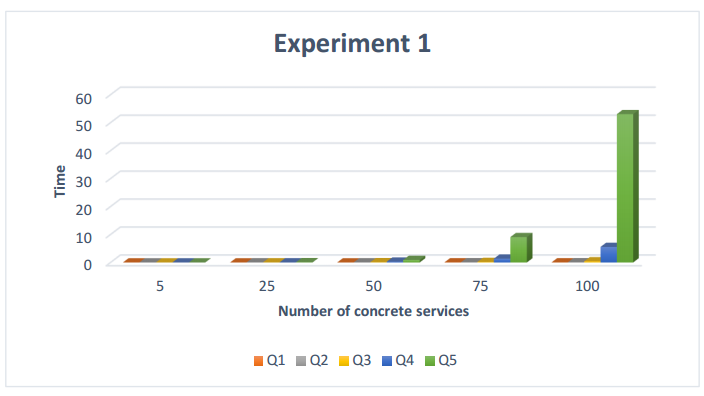
\includegraphics[scale=0.4]{exp1.png}
\caption{Query rewriting evaluation.}\label{fig01}
\end{figure} 

In the \textit{experiment 1}, there are five different queries that differ on the quantity of abstract services (increasing from 2 to 6). Analyzing the first experiment, it is easily to identify that the algorithm shares the same problem as existing query rewriting approaches using views: increasing the processing time when the size of the query and the number of concrete services increase. 

\begin{figure}[!h]
\centering
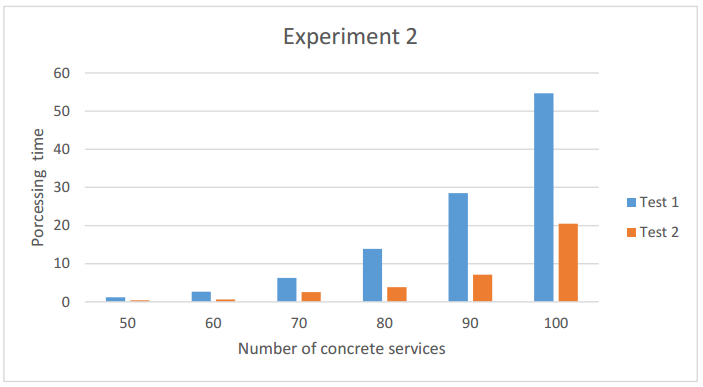
\includegraphics[scale=0.4]{exp2.png}
\caption{Query rewriting evaluation.}\label{fig02}
\end{figure} 

The \textit{experiment 2} presents the results considering our contribution regarding the use of user preferences and services' quality aspects extracted from SLAs to guide the service selection and query rewriting.
\textit{Test 1} and \textit{Test 2} include queries with six abstract services. 
The important difference between them is use of quality measures guiding the process. \textit{Test 1} do not consider quality measures as any other existing rewriting approach. On the other hand, \textit{Test 2} considers them.
The figure~\ref{fig02} shows our results. 

\begin{figure}[!h]
\centering
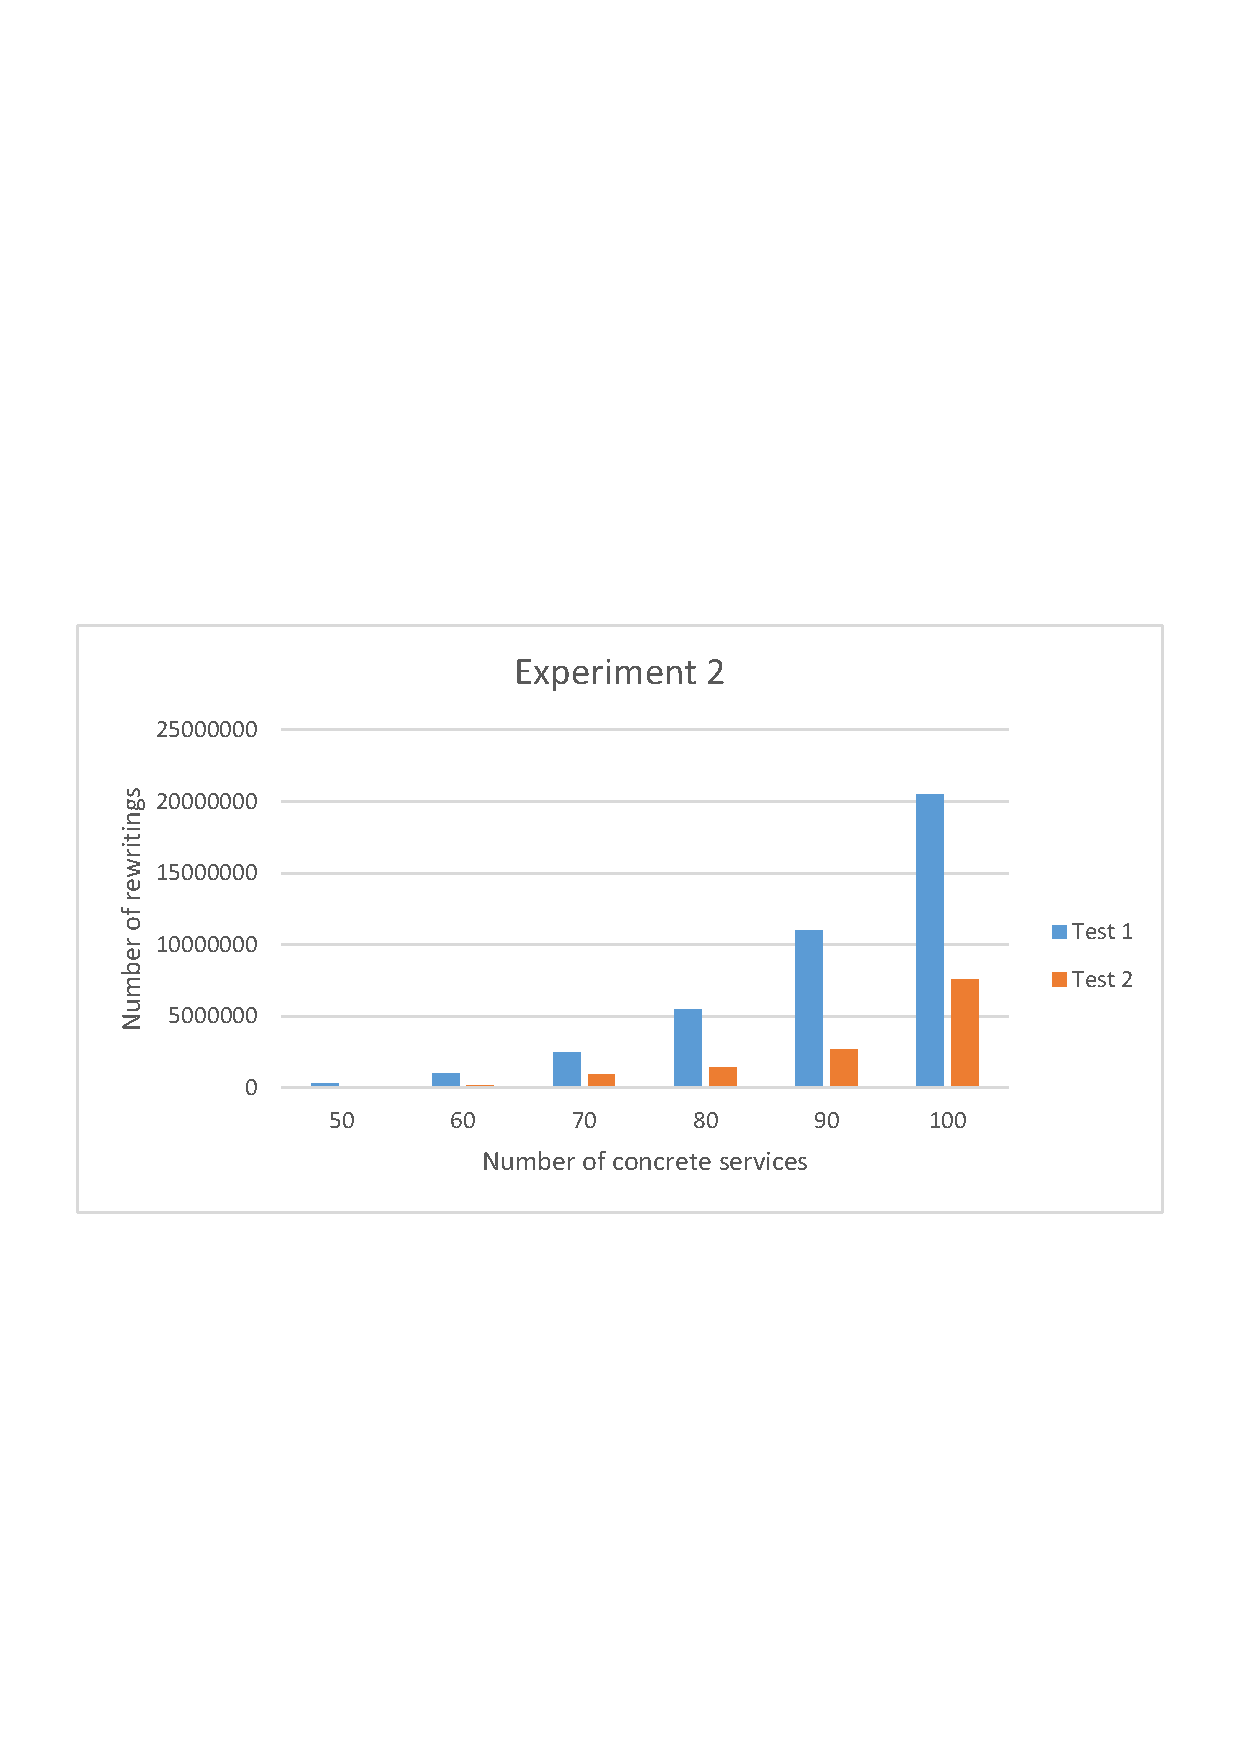
\includegraphics[scale=0.4]{exp3.png}
\caption{Query rewriting evaluation.}\label{fig03}
\end{figure} 

Analyzing the \textit{experiment 2}, the results while considering the quality measures are promising.  
%The \textit{Rhone} presents a better performance, decreasing the processing time and 
%the total number of rewritings produced.  
%Reducing rewriting number allow to go straightforward to the rewriting solutions that are satisfactory avoiding any further backtrack.
The \textit{Rhone} increases performance reducing rewriting number which allows to go straightforward to the rewriting solutions that are satisfactory avoiding any further backtrack and thus reducing successful integration time.